\documentclass{article}



\usepackage[brazil]{babel}

\usepackage[utf8]{inputenc}

\usepackage{amsmath}

\usepackage{amsfonts}



\usepackage[section]{placeins}



\usepackage{graphicx}



\usepackage{color} %red, green, blue, yellow, cyan, magenta, black, white

\definecolor{mygreen}{RGB}{28,172,0} % color values Red, Green, Blue

\definecolor{mylilas}{RGB}{170,55,241}



\begin{document}



\begin{flushleft}

\textbf{FUNDAÇÃO GETÚLIO VARGAS} \\



\textbf{Escola de Pós-Graduação em Economia}



\textbf{Teoria Macroeconômica III - Lista 04}



Professor: Ricardo de Oliveira Cavalcanti



Monitora: Kátia Aiko Nishiyama Alves



Alunos: Gustavo Bulhões e Samuel Barbosa

\end{flushleft}



\section*{Exercício 01}

Neste exercício consideramos o modelo bancário de Diamond \& Dybvig com os objetos básicos dados no enunciado. 



\subsection*{Item (a)}

A matriz de coeficientes $F$ calculada é: 
\\
\\
\begin{center}

$F
=
\begin{bmatrix}
    1.9760 & 0.9880 & 0  \\
    0 & 1.9639 & 0.9759 \\
    0 & 0 & 1.9519 
\end{bmatrix}
$

\end{center}


\subsection*{Item (b)}

Vide código do MATLAB anexo.


\subsection*{Item (c)}

Em autarquia, os indivíduos não realizam depósitos junto ao intermediário bancário, o que faz com que a matriz de coeficientes associada seja constituída apenas por elementos nulos.
\\
\\
\begin{center}

$F_{autarquia}
=
\begin{bmatrix}
    0 & 0 & 0  \\
    0 & 0 & 0 \\
    0 & 0 & 0
\end{bmatrix}
$

\end{center}



\subsection*{Item (d)}

Encontramos que o bem-estar da sociedade sob autarquia e sob o mecanismo ótimo é o mesmo: $-0.0976$. Logo, considerando que ao estarem indiferentes os indivíduos optam pelo mecanismo ótimo, os mesmos aceitam participar do arranjo bancário. 

\subsection*{Item (e)}

Encontramos que o bem-estar ex-post em uma corrida bancária é de $-0.1$, ou seja, é pior do que ambos os casos de autarquia e do mecanismo ótimo. 


\subsection*{Item (f)}

Podemos ver que, embora em valor absoluto as diferenças sejam pequenas (4 ou 5 casas decimais), o bem estar em autarquia permanece o mesmo, enquanto o bem estar do mecanismo ótimo aumenta com o aumento de N, reforçando que os indivíduos sempre escolhem participar do arranjo bancário. O resultado mostra que quanto maior for N, maiores são os ganhos que os indivíduos têm de realizar depósitos junto ao intermediário bancário.

\begin{figure}[!h]

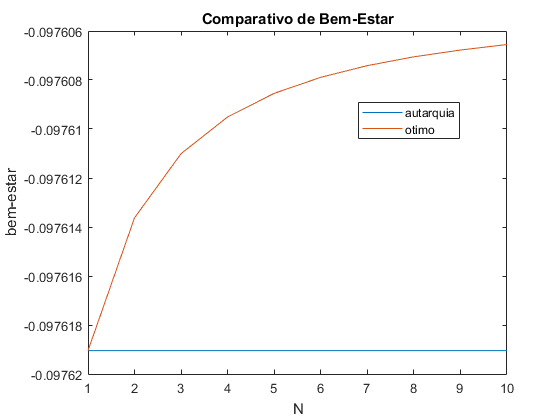
\includegraphics[scale=0.6]{Ex1/ex1_1.png}

\end{figure}


\section*{Exercício 02}

\subsection*{Item (a)}

Sob o mecanismo ótimo para economia da questão anterior, com $N=2$ e $A=1$, obtemos que
a utilidade esperada do agente paciente de anunciar seu tipo verdadeiro é maior do que a de se passar por impaciente
$(-0.0961 > -0.1000)$, mesmo se acredita que os demais pacientes irão mentir. Teremos um equilíbrio de \textit{truth-telling}
(estratégias dominantes), o que afasta a possibilidade de haver corrida bancária. 

\subsection*{Item (b)}

Ao variar os valores para o parâmentro $A$, observamos que a decisão ótima do agente 
paciente se altera. Em especial, quando $A \geq 1.25$, o resultado do item anterior
deixa de valer e passamos a ter corrida bancária.

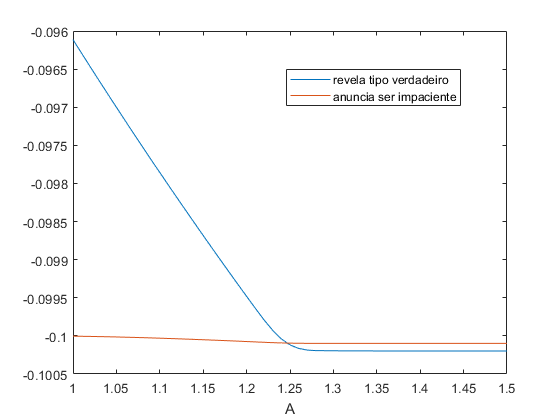
\includegraphics[scale=0.6]{Ex1/ex2_1.png}

\subsection*{Item (c)}

Mantendo $A = 1$ fixo e variando $N$, observamos que com $N \geq 35$ também
passamos a ter corrida bancária.

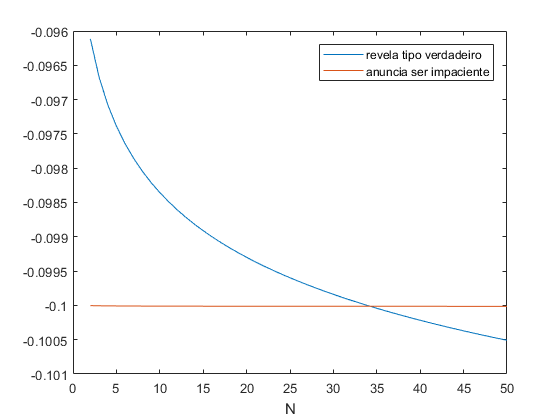
\includegraphics[scale=0.6]{Ex1/ex2_2.png}


\end{document}
